\documentclass{beamer}

\usepackage[utf8]{inputenc}
\usepackage[brazilian]{babel}
\usepackage{amsmath}
\usepackage{enumerate}
\usepackage[]{graphicx}
\usepackage{subfigure}
\usepackage[]{color}
\usepackage{pgfplots}
\usepackage{systeme}
\usepackage{listings}
\usetheme{Berkeley}

%Define estilo para o código
\definecolor{codegreen}{rgb}{0,0.6,0}
\definecolor{codegray}{rgb}{0.5,0.5,0.5}
\definecolor{codepurple}{rgb}{0.58,0,0.82}
\definecolor{backcolour}{rgb}{0.95,0.95,0.92}

\lstdefinestyle{mystyle}{
	backgroundcolor=\color{backcolour},   
	commentstyle=\color{codegreen},
	keywordstyle=\color{magenta},
	numberstyle=\tiny\color{codegray},
	stringstyle=\color{codepurple},
	basicstyle=\footnotesize,
	breakatwhitespace=false,         
	breaklines=true,                 
	captionpos=b,                    
	keepspaces=true,                 
	numbers=left,                    
	numbersep=5pt,                  
	showspaces=false,                
	showstringspaces=false,
	showtabs=false,                  
	tabsize=2
}

\lstset{style=mystyle}



\begin{document}
	\title{Relevância de Textos com Lógica Fuzzy}
	\author{\textit{Eric Calasans de Barros \and José Genilson da Silva Filho}}
	\institute{Universidade Federal do Rio Grande do Norte}
	
	\section{Capa}
	\begin{frame}[plain]
		\maketitle
	\end{frame}
	
	\section{Introdução}
	\begin{frame}{Introdução}
		\begin{itemize}
			\item \textbf{Natural Language Processing(NLP)}\\
			\item \textbf{Classificação de Texto}\\
			\item \textbf{Perspectivas de Personalidade}\\
			\item \textbf{Classificação de Emoção}
		\end{itemize}
	\end{frame}
	
	\section{Metodologia}
	\begin{frame}{Metodologia}
				\textbf{\large Ferramentas Utilizadas}
				\begin{itemize}
					\item \textbf{Python:}\\
							\texttt{nltk} - para análise e processamento do texto\\
							\texttt{skfuzzy} - para calcular relevância do texto através da lógica fuzzy\\
							
					\item \textbf{Textos para validação} - \texttt{futebol.txt} e \texttt{medicina.txt}
				\end{itemize}
	\end{frame}
	\begin{frame}[fragile]{Metodologia}
\begin{lstlisting}[language=Python, caption = Preparação do Texto]
stemmer = RSLPStemmer() #extracao dos radicais das palavras					
palavras = ['jogador', 'futebol'] # dicionario					
arquivo = open('medicina.txt', 'r') #abrindo o arquivo					
texto = arquivo.read() \# texto a ser comparado					
words = (nltk.word_tokenize(texto)) #texto tokenrizsdo					
stops = set(stopwords.words("portuguese")) #conjunto de palavras sem importancia para a classificacao do texto					
word_features = ([w for w in words if not w in stops]) #stop words removioda do texto
\end{lstlisting}
	\end{frame}
	
	\begin{frame}{Metodologia}
		\textbf{\large Cálculo dos Matchs}
		\begin{itemize}
			\item \textbf{Match Total}$$matchTotal_{i} = \frac{nOcorrCompleta_{i}}{\sum_{i=1}^{n} nOcorrCompleta_{i}}$$
			\item \textbf{Match Radical}$$matchRadical_{i} = \frac{nOcorrRad_{i}}{\sum_{i=1}^{n} nOcorrRad{i}}$$
			\item \textbf{\textit{No Match}}$$noMatch_{i} = \frac{ausRad_{i}}{\sum_{i=1}^{n} ausRad_{i}}$$
		\end{itemize}
	\end{frame}
	\begin{frame}[fragile]{Metodologia}
\begin{lstlisting}[language=Python, caption = Match total]
#Procurando match total
def matchWord(texto, dicionario):
	bag_words ={} # Inicia o dicionario que vai guardar os matchs do dicionario no texto
	for i in dicionario:
		bag_words[i] = 0
# Procura os matchs entre o dicionario e o texto; incrementa +1 quando encontra na chave do dicionario que
# se refere a palavra que esta sendo analisada
	for palavraTexto in texto:
		for palavraDicionario in dicionario:
			if (palavraTexto == palavraDicionario):
				bag_words[palavraDicionario] +=1

	return(bag_words)
\end{lstlisting}
	\end{frame}

	\begin{frame}[fragile]{Metodologia}
\begin{lstlisting}[language=Python, caption = Match de radical]
# Procurando match de radical
def macthRadical(texto, dicionario):
	textoStemmer = [stemmer.stem(w.lower()) for w in texto] # Transforma as palavras do dicionario em radicais
	dicStermmer = [stemmer.stem(w.lower()) for w in dicionario] # Transforma as palavras do texto em radicais
	bag_words ={}
	nMatch = {}  # Palavras que nao concordam com o radical
	# Inicia o dicionario que sera usado para contabilizar os radicais e as palavras que nao tiveram match
	for i in dicStermmer:
		bag_words[i] = 0
		nMatch[i] = 0
\end{lstlisting}
	\end{frame}

	\begin{frame}[fragile]{Metodologia}
\begin{lstlisting}[language=Python, caption = Match de radical(cont.)]
	# Procura os radicais como feito no metodo anterior
	for palavraTexto in textoStemmer:
		for palavraDicionario in dicStermmer:
			if (palavraTexto == palavraDicionario):
				bag_words[palavraDicionario] += 1
				
	# Procura as palavras que nao estao presente no texto e estao no dicionario
	for palavraDicionario in dicStermmer:
		if (not palavraDicionario in textoStemmer):
			nMatch[palavraDicionario] += 1
				
	return(bag_words, nMatch)
\end{lstlisting}
	\end{frame}

	\begin{frame}[fragile]{Metodologia}
\begin{lstlisting}[language=Python, caption = Relevância de cada palavra]
#Relevancia de uma palavra	
def relevancia():
	#Inicializacoes
	total = matchWord(word_features, palavras)
	radical, nMatch = macthRadical(word_features, palavras)
	
	relevancia_total_sum = 0
	relevancia_radical_sum = 0
	relevancia_nMatch_sum = 0	
	\end{lstlisting}
\end{frame}

	\begin{frame}[fragile]{Metodologia}
\begin{lstlisting}[language=Python, caption = Relevância de cada palavra(cont.)]
	for matchPalavra, key in enumerate(total):
		if(relevancia_total_sum == 0):
			relevancia_total_sum = 1
		relevancia_total[key] = total[key]/relevancia_total_sum
	
	for matchPalavra, key in enumerate(radical):
		if(relevancia_radical_sum == 0):
			relevancia_radical_sum = 1        
		relevancia_radical[key] = radical[key]/relevancia_radical_sum
\end{lstlisting}
	\end{frame}

	\begin{frame}[fragile]{Metodologia}
\begin{lstlisting}[language=Python, caption = Relevância de cada palavra(cont.)]
	for matchPalavra, key in enumerate(nMatch):
		if(relevancia_nMatch_sum == 0):
			relevancia_nMatch[key] = 0
		else:
			if(relevancia_nMatch_sum == 0):
				relevancia_nMatch_sum = 1
			relevancia_nMatch[key] = nMatch[key]/relevancia_nMatch_sum
\end{lstlisting}
	\end{frame}	

	\begin{frame}[fragile]{Metodologia}
\begin{lstlisting}[language=Python, caption = Relevância de uma palavra(cont.)]
	print(relevancia_total)
	print(relevancia_radical)
	print(relevancia_nMatch)
	
	return(relevancia_total, relevancia_radical, relevancia_nMatch)
\end{lstlisting}
	\end{frame}

	\begin{frame}[fragile]{Metodologia}
\begin{lstlisting}[language=Python, caption = Lógica Fuzzy]
def fuzzyRelText(relTotal=0, relRadical=0, relNoMatch=0):
	# Cria as variaveis fuzzy:  Antecedentes e Consequente
	# Antecedentes
	total = ctrl.Antecedent(np.arange(start=0, stop=1.1, step=0.1), 'Total')
	radical = ctrl.Antecedent(np.arange(start=0, stop=1.1, step=0.1), 'Radical')
	noMatch = ctrl.Antecedent(np.arange(start=0, stop=1.1, step=0.1), 'NoMatch')
	
	#Consequente
	nivelRelevancia = ctrl.Consequent(np.arange(start=0.0, stop=1.1, step=0.1), 'Relevancia')
\end{lstlisting}
	\end{frame}

	\begin{frame}[fragile]{Metodologia}
\begin{lstlisting}[language=Python, caption = Lógica Fuzzy]
	#Funcoes
	#Total
	total['nRelevante'] = fuzzy.trimf(total.universe, [0, 0, 0.8])
	total['relevante'] = fuzzy.trimf(total.universe, [0.2, 1, 1])
	
	#Radical
	radical['nRelevante'] = fuzzy.trimf(radical.universe, [0, 0, 0.8])
	radical['relevante'] = fuzzy.trimf(radical.universe, [0.2, 1, 1])
\end{lstlisting}
	\end{frame}

	\begin{frame}[fragile]{Metodologia}
\begin{lstlisting}[language=Python, caption = Lógica Fuzzy(cont.)]	
	#NoMatch
	noMatch['nRelevante'] = fuzzy.trimf(noMatch.universe, [0, 0, 0.8])
	noMatch['relevante'] = fuzzy.trimf(noMatch.universe, [0.2, 1, 1])
	
	#resultado
	nivelRelevancia['poucoRelevante'] = fuzzy.trimf(nivelRelevancia.universe, [0, 0, 0.4])
	nivelRelevancia['relevante'] = fuzzy.trimf(nivelRelevancia.universe, [0.1, 0.5, 0.9])
	nivelRelevancia['muitoRelevante'] = fuzzy.trimf(nivelRelevancia.universe, [0.6, 1, 1])
\end{lstlisting}
	\end{frame}	

	\begin{frame}[fragile]{Metodologia}
\begin{lstlisting}[language=Python, caption = Lógica Fuzzy(cont.)]	
	# Regras
	r1 = ctrl.Rule(antecedent=total['relevante'] & radical['relevante'] & noMatch['nRelevante'],
					consequent=nivelRelevancia['muitoRelevante'])
	r2 = ctrl.Rule(antecedent=total['nRelevante'] & radical['nRelevante'] & noMatch['relevante'],
					consequent=nivelRelevancia['poucoRelevante'])
	r3 = ctrl.Rule(antecedent=total['relevante'] & radical['relevante'] & noMatch['nRelevante'],
					consequent=nivelRelevancia['relevante']%0.8)
	r4 = ctrl.Rule(antecedent=total['relevante'] & radical['relevante'] & noMatch['relevante'],
					consequent=nivelRelevancia['relevante']%0.6)

\end{lstlisting}
	\end{frame}	

	\begin{frame}[fragile]{Metodologia}
\begin{lstlisting}[language=Python, caption = Lógica Fuzzy(cont.)]	
	# Regras
	r5 = ctrl.Rule(antecedent=total['relevante'] & radical['nRelevante'] & noMatch['nRelevante'],
					consequent=nivelRelevancia['relevante']%0.7)
	r6 = ctrl.Rule(antecedent=total['nRelevante'] & radical['relevante'] & noMatch['nRelevante'],
					consequent=nivelRelevancia['relevante']%0.5)
	r7 = ctrl.Rule(antecedent=total['nRelevante'] & radical['nRelevante'] & noMatch['nRelevante'],
		consequent=nivelRelevancia['poucoRelevante'])
\end{lstlisting}
	\end{frame}	

	\begin{frame}[fragile]{Metodologia}
\begin{lstlisting}[language=Python, caption = Lógica Fuzzy(cont.)]	
	#Cria maquina de inferencia
	controleRelevancia = ctrl.ControlSystem([r1, r2, r3, r4, r5, r6, r7])
	
	#Prepara a simulacao
	resultado = ctrl.ControlSystemSimulation(control_system=controleRelevancia)
	
	#Entrada de dados
	resultado.input['Total'] = relTotal
	resultado.input['Radical'] = relRadical
	resultado.input['NoMatch'] = relNoMatch
\end{lstlisting}
	\end{frame}	

	\begin{frame}[fragile]{Metodologia}
\begin{lstlisting}[language=Python, caption = Resultado final]	
	#Defuzzificacao
	resultado.compute()
	
	#Retorna relevancia
	return resultado.output['Relevancia']
\end{lstlisting}
	\end{frame}

	\begin{frame}[fragile]{Metodologia}
\begin{lstlisting}[language=Python, caption = Lógica Fuzzy(cont.)]	
(total, radical, nMatch) = relevancia()
rele = 0
	
# A relevancia final do texto e calculada somando as relevancias de cada palavra do dicionario dividido pela quantidade
# de palavras no dicionario
for word, key in enumerate(total):
	rele += fuzzyText.fuzzyRelText(total[key], radical[stemmer.stem(key)], nMatch[stemmer.stem(key)])
	
print(rele/len(total))  
\end{lstlisting}
	\end{frame}
	
	\section{Resultados}
	\begin{frame}{Resultados}
		\textbf{Texto }\texttt{futebol.txt}\\
		\texttt{\tiny Há relatos de um esporte muito parecido com o futebol, embora usava-se muito a violência. O Soule ou Harpastum era praticado na Idade Média por militares que se dividiam em duas equipes: atacantes e defensores. Era permitido usar socos, pontapés, rasteiras e outros golpes violentos. Há relatos que mostram a morte de alguns jogadores durante a partida. Cada equipe era formada por 27 jogadores, onde grupos tinham funções diferentes no time: corredores, dianteiros, sacadores e guarda-redes.
			Na Itália Medieval apareceu um jogo denominado gioco del calcio. Era praticado em praças e os 27 jogadores de cada equipe deveriam levar a bola até os dois postes que ficavam nos dois cantos extremos da praça. A violência era muito comum, pois os participantes levavam para campo seus problemas causados, principalmente por questões sociais típicas da época medieval. 
			O barulho, a desorganização e a violência eram tão grandes que o rei Eduardo II teve que decretar uma lei proibindo a prática do jogo, condenando a prisão os praticantes. Porém, o jogo não terminou, pois integrantes da nobreza criaram uma nova versão dele com regras que não permitiam a violência. Nesta nova versão, cerca de doze juízes deveriam fazer cumprir as regras do jogo.
			}  
	\end{frame}
	
	\begin{frame}{Resultados}
		\begin{itemize}
			\item \textbf{Dicionário:  }\texttt{jogador;  futebol}\\
			\item \textbf{Texto:  } \texttt{futebol.py}
			\item \textbf{Matches:  } 
				\begin{align*}
					\text{'futebol'} \rightarrow &total = 1.0, radical = 0.125 \text{ e } noMatch = 0\\
					\text{'jogador'} \rightarrow &total = 0.0, radical = 0.875 \text{ e } noMatch = 0
				\end{align*}
		\end{itemize}
	\end{frame}
	
	\begin{frame}
		\begin{figure}[H]
			\centering
			\subfigure{
				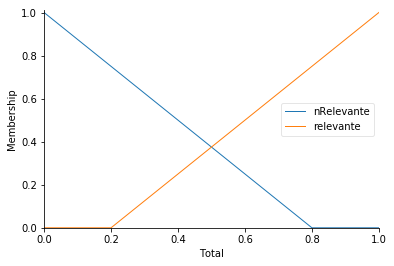
\includegraphics[width=0.4\linewidth]{futebolFutTotal}
			}
			~
			\subfigure{
				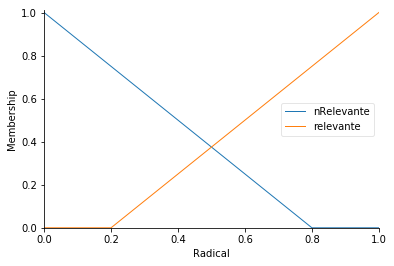
\includegraphics[width=0.4\linewidth]{futebolFutRadical}
			}
			~
			\subfigure{
				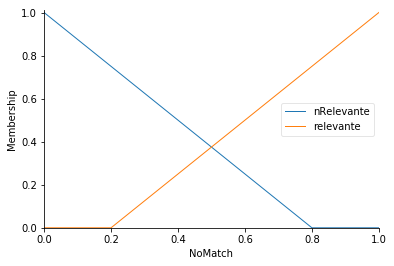
\includegraphics[width=0.4\linewidth]{futebolFutNoMatch}
			}
			~
			\subfigure{
				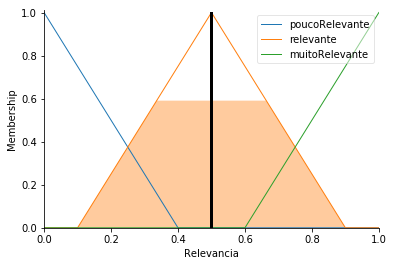
\includegraphics[width=0.4\linewidth]{futebolFutNR}
			}
			\caption{Palavra 'futebol' no texto \texttt{futebol.txt}}	
		\end{figure}
	\end{frame}
	
		\begin{frame}
	\begin{figure}[H]
		\centering
		\subfigure{
			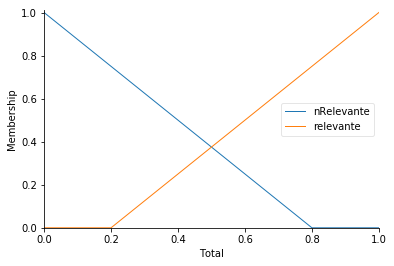
\includegraphics[width=0.4\linewidth]{jogadorFutTotal}
		}
		~
		\subfigure{
			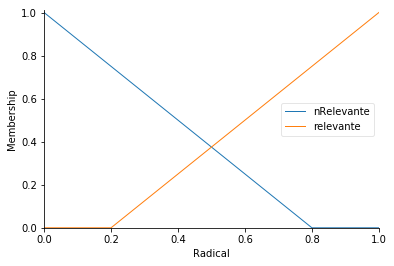
\includegraphics[width=0.4\linewidth]{jogadorFutRadical}
		}
		~
		\subfigure{
			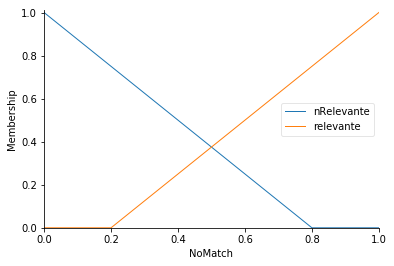
\includegraphics[width=0.4\linewidth]{jogadorFutNoMatch}
		}
		~
		\subfigure{
			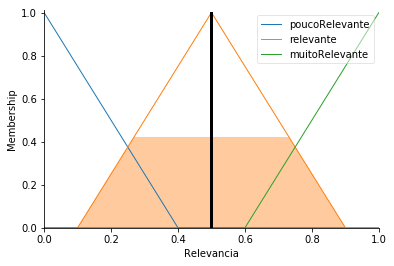
\includegraphics[width=0.4\linewidth]{jogadorFutNR}
		}
		\caption{Palavra 'jogador' no texto \texttt{futebol.txt}}	
	\end{figure}
\end{frame}
	
	\begin{frame}{Resultados}
		\textbf{Texto }\texttt{medicina.txt}\\
		\texttt{\tiny A medicina é uma das muitas áreas do conhecimento ligada à manutenção e restauração da saúde. Ela trabalha, num sentido amplo, com a prevenção e cura das doenças humanas e animais num contexto médico.
			Ações de saúde pública e ambiental, incluindo a saúde animal, promoção, prevenção, controle, erradicação e tratamento das doenças, traumatismos ou qualquer outro agravo à integridade e bem-estar animais, além do controlo de sanidade dos produtos e subprodutos de origem animal para o consumo humano e animal compreendem a área da medicina da responsabilidade do profissional de saúde médico veterinário.
			Em Portugal, a saúde oral, higiene, integridade dentária, a sua limpeza e profilaxia compreendem a área da medicina da responsabilidade do Médico Dentista, que é um profissional da saúde capacitado na área de odontologia, e apesar de ter um âmbito de acção semelhante, não deve ser confundido com o Médico estomatologista. Porém no Brasil, odontologia e medicina são profissões distintas.
			Segundo a Organização Mundial da Saúde, saúde não é apenas a ausência de doença. Consiste no bem-estar físico, mental, psicológico e social do indivíduo. }
	\end{frame}
	
	\begin{frame}{Resultados}
		\texttt{\tiny É um estado cumulativo, que deve ser promovido durante toda a vida, de maneira a assegurar-se de que seus benefícios sejam integralmente desfrutados em dias posteriores. Nesse contexto, diretrizes de organizações supra-nacionais compostas por eminentes intelectuais do globo relacionados à área de saúde estabeleceram um novo paradigma de abordagem em medicina. O santo patrono da Medicina é São Lucas.}
	\end{frame}
	
	
	\begin{frame}{Resultados}
		\begin{itemize}
			\item \textbf{Dicionário:  }\texttt{jogador;  futebol}\\
			\item \textbf{Texto:  } \texttt{medicina.py}
			\item \textbf{Matches:  } 
				\begin{align*}
					\text{'futebol'} \rightarrow &total = 1.0, radical = 0.125 \text{ e } noMatch = 0\\
					\text{'jogador'} \rightarrow &total = 0.0, radical = 0.875 \text{ e } noMatch = 0
				\end{align*}
		\end{itemize}
	\end{frame}

	\begin{frame}
		\begin{figure}[H]
			\centering
			\subfigure{
				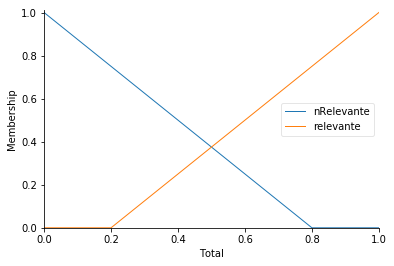
\includegraphics[width=0.4\linewidth]{futebolMedTotal}
			}
			~
			\subfigure{
				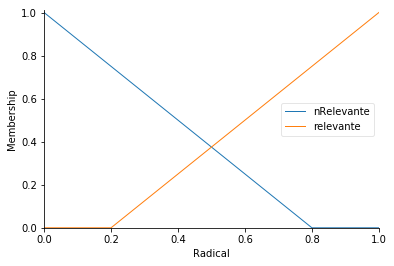
\includegraphics[width=0.4\linewidth]{futebolMedRadical}
			}
			~
			\subfigure{
				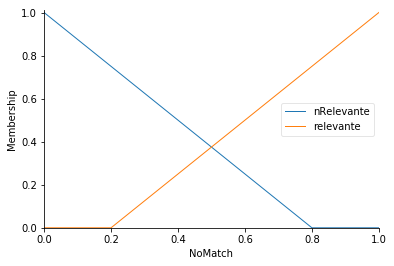
\includegraphics[width=0.4\linewidth]{futebolMedNoMatch}
			}
			~
			\subfigure{
				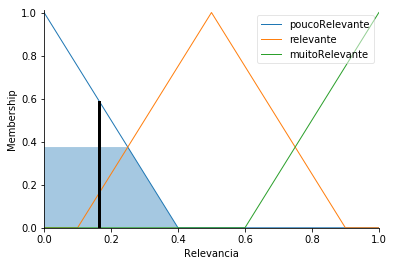
\includegraphics[width=0.4\linewidth]{futebolMedNR}
			}
			\caption{Palavra 'futebol' no texto \texttt{medicina.txt}}	
		\end{figure}
	\end{frame}

	\begin{frame}
		\begin{figure}[H]
			\centering
			\subfigure{
				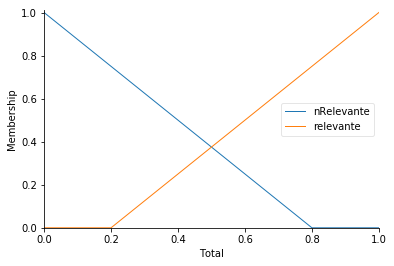
\includegraphics[width=0.4\linewidth]{futebolMedTotal}
			}
			~
			\subfigure{
				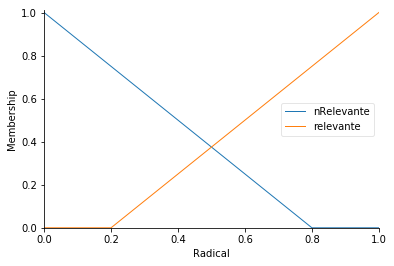
\includegraphics[width=0.4\linewidth]{futebolMedRadical}
			}
			~
			\subfigure{
				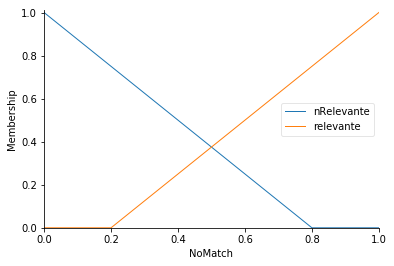
\includegraphics[width=0.4\linewidth]{futebolMedNoMatch}
			}
			~
			\subfigure{
				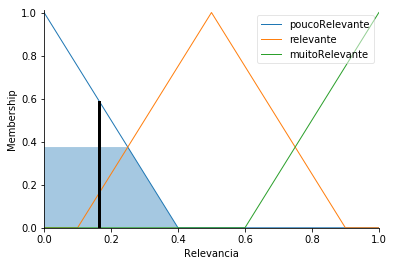
\includegraphics[width=0.4\linewidth]{futebolMedNR}
			}
			\caption{Palavra 'jogador' no texto \texttt{medicina.txt}}	
		\end{figure}
	\end{frame}

	\begin{frame}[plain]
		\centering
		\Large Conclusões
	\end{frame}
	
\end{document}